\documentclass{article}
\usepackage{amsmath}
\usepackage{amsfonts}
\usepackage{amssymb}
\usepackage{cancel}

\usepackage{graphicx}


\setlength\parindent{0pt}

\author{Pranav Tikkawar}
\title{Workshop 7}

\begin{document}
\maketitle
\section*{Question 2}
Find the motion through the intial point $\begin{bmatrix}
    1\\
    1\\
    2\\
\end{bmatrix}$ if $ A = \begin{bmatrix}
    6 & -8 & -7 \\
    3 & -3 & -3 \\
    3 & -2 & -4 \\
\end{bmatrix}$ \\
Eigenvalues of the matrix is given by $A - \lambda I = \begin{bmatrix}
    6 - \lambda & -8 & -7 \\
    3 & -3 - \lambda & -3 \\
    3 & -2 & -4 - \lambda \\
\end{bmatrix} $
The charecteristic polynomial of the matrix is given by
$$(-6 - \lambda)[(-3-\lambda)(-4-\lambda) - 6] + 8[3(-4-\lambda) + 9] - 7[-3(-3-\lambda) - 6] $$
The charecteristic polynomial simplifies to $$-\lambda^3 - \lambda^2 -9 \lambda - 9$$
$$(-1 - \lambda)(\lambda^2 + 9)$$
Thus the eigenvalues of the matrix is given by $\mu_1 = -1, \mu_2 = 3i, \mu_3 = -3i$.\\
The eigenvector for the eigenvalue $\mu_1 = -1$ is given by solving the equation $(A - \mu_1 I)X = 0$. Here the matrix $[A - \mu_1 I | 0]$ is given by
$$\begin{bmatrix}
    7 & -8 & -7 & 0\\
    3 & -2 & -3 & 0\\
    3 & -2 & -3 &0
\end{bmatrix} $$
The reduced row echelon form of the matrix is
$$\begin{bmatrix}
    1 & 0 & -1 & 0\\
    0 & 1 & 0 & 0\\
    0 & 0 & 0 & 0 
\end{bmatrix} $$
Thus the eigenvector for the eigenvalue $\mu_1 = -1$ is given by
$$\begin{bmatrix}
    1\\
    0\\
    1
\end{bmatrix} $$
The eigenvector for the eigenvalue $\mu_2 = 3i$ is given by solving the equation $(A - \mu_2 I)X = 0$. Here the matrix $[A - \mu_2 I | 0]$ is given by
$$\begin{bmatrix}
    6 - 3i & -8 & -7 & 0\\
    3 & -3 - 3i & -3 & 0\\
    3 & -2 & -4 - 3i & 0
\end{bmatrix} $$
The reduced row echelon form of the matrix is
$$\begin{bmatrix}
    0 & 1+3i & -1-3i & 0\\
    1 & -1-i & -1 & 0\\
    0 & 1+3i & -1-3i & 0
\end{bmatrix}, \begin{bmatrix}
    1 & -1-i & -1 & 0\\
    0 & 1+3i & -1-3i & 0\\
    0 & 0 & 0 & 0
\end{bmatrix}, \begin{bmatrix}
    1 & 0 & -2-i & 0\\
    0 & 1 & -1 & 0\\
    0 & 0 & 0 & 0
\end{bmatrix}$$
Thus the eigenvector for the eigenvalue $\mu_2 = 3i$ is given by
$$\begin{bmatrix}
    2+i\\
    1\\
    1
\end{bmatrix} $$
Therefore we can split up this eigenvector into two vectors, one for the real part and one for the imaginary part. Thus the eigenvector for the eigenvalue $\mu_2 = 3i$ is given by
$$\begin{bmatrix}
    2\\
    1\\
    1
\end{bmatrix} + i\begin{bmatrix}
    1\\
    0\\
    0
\end{bmatrix} $$
And $x=e^{3it}x_0$ is given by $[cos(3t) + isin(3t)]\begin{bmatrix}
    2 +i \\
    1\\
    1
\end{bmatrix} $ for the first 2 rows \\
Thus the solution to the system of differential equations is given by
$$\begin{bmatrix}
    2cos(3t) - sin(3t)\\
    cos(3t)\\
    cos(3t)
\end{bmatrix} + \begin{bmatrix}
    cos(3t)+2sin(3t)\\
    sin(3t)\\
    sin(3t)
\end{bmatrix}$$
Therefore our $M(t)$ is given by
$$\begin{bmatrix}
    2cos(3t) - sin(3t) & cos(3t)+2sin(3t) & e^{-t}\\
    cos(3t) & sin(3t) & 0\\
    cos(3t) & sin(3t) & e^{-t}
\end{bmatrix}$$
Our $M(0)$ is given by
$$\begin{bmatrix}
    2 & 1 & 1\\
    1 & 0 & 0\\
    1 & 0 & 1
\end{bmatrix}$$
The inverse $M(0)^{-1}$ is given by: $$\begin{bmatrix}
    0 & 1 & 0\\
    1 & -1 & -1\\
    0 & -1 & 1
\end{bmatrix}$$
Thus the new matrix $G(t)$ which solves $Y(t) = G(t)Y^{(0)}$ is given by
$$\begin{bmatrix}
    2cos(3t) - sin(3t) & cos(3t)+2sin(3t) & e^{-t}\\
    cos(3t) & sin(3t) & 0\\
    cos(3t) & sin(3t) & e^{-t}
\end{bmatrix} \begin{bmatrix}
    0 & 1 & 0\\
    1 & -1 & -1\\
    0 & -1 & 1
\end{bmatrix}$$
When considering the intial condition: $\begin{bmatrix}
    1\\
    1\\
    2\\
\end{bmatrix}$, we get the solution to the system of differential equations as
$$\begin{bmatrix}
    2cos(3t) - sin(3t) & cos(3t)+2sin(3t) & e^{-t}\\
    cos(3t) & sin(3t) & 0\\
    cos(3t) & sin(3t) & e^{-t}
\end{bmatrix} \begin{bmatrix}
    0 & 1 & 0\\
    1 & -1 & -1\\
    0 & -1 & 1
\end{bmatrix} \begin{bmatrix}
    1\\
    1\\
    2\\
\end{bmatrix}$$
$$ = \begin{bmatrix}
    2cos(3t) - sin(3t) & cos(3t)+2sin(3t) & e^{-t}\\
    cos(3t) & sin(3t) & 0\\
    cos(3t) & sin(3t) & e^{-t}
\end{bmatrix} \begin{bmatrix}
    1\\
    -2\\
    1\\
\end{bmatrix}$$
$$= \begin{bmatrix}
    2cos(3t) - sin(3t) - 2cos(3t) -4sin(3t) + e^{-t}\\
    cos(3t) - 2sin(3t)\\
    cos(3t) - 2sin(3t) + e^{-t}
\end{bmatrix}$$
$$= \begin{bmatrix}
    -5sin(3t) + e^{-t}\\
    cos(3t) - 2sin(3t)\\
    cos(3t) - 2sin(3t) + e^{-t}
\end{bmatrix}$$
Given as a sum of Periodic and non-Periodic terms is
$$\begin{bmatrix}
    -5sin(3t)\\
    cos(3t) - 2sin(3t)\\
    cos(3t) - 2sin(3t)
\end{bmatrix} + \begin{bmatrix}
    e^{-t}\\
    0\\
    e^{-t}
\end{bmatrix}$$
The limit as $t \to \infty$ is going to be a Periodic motion. since the non-periodic term will tend to 0 as $t \to \infty$ and the periodic term will remain and continue to oscillate.\\


\begin{center}
    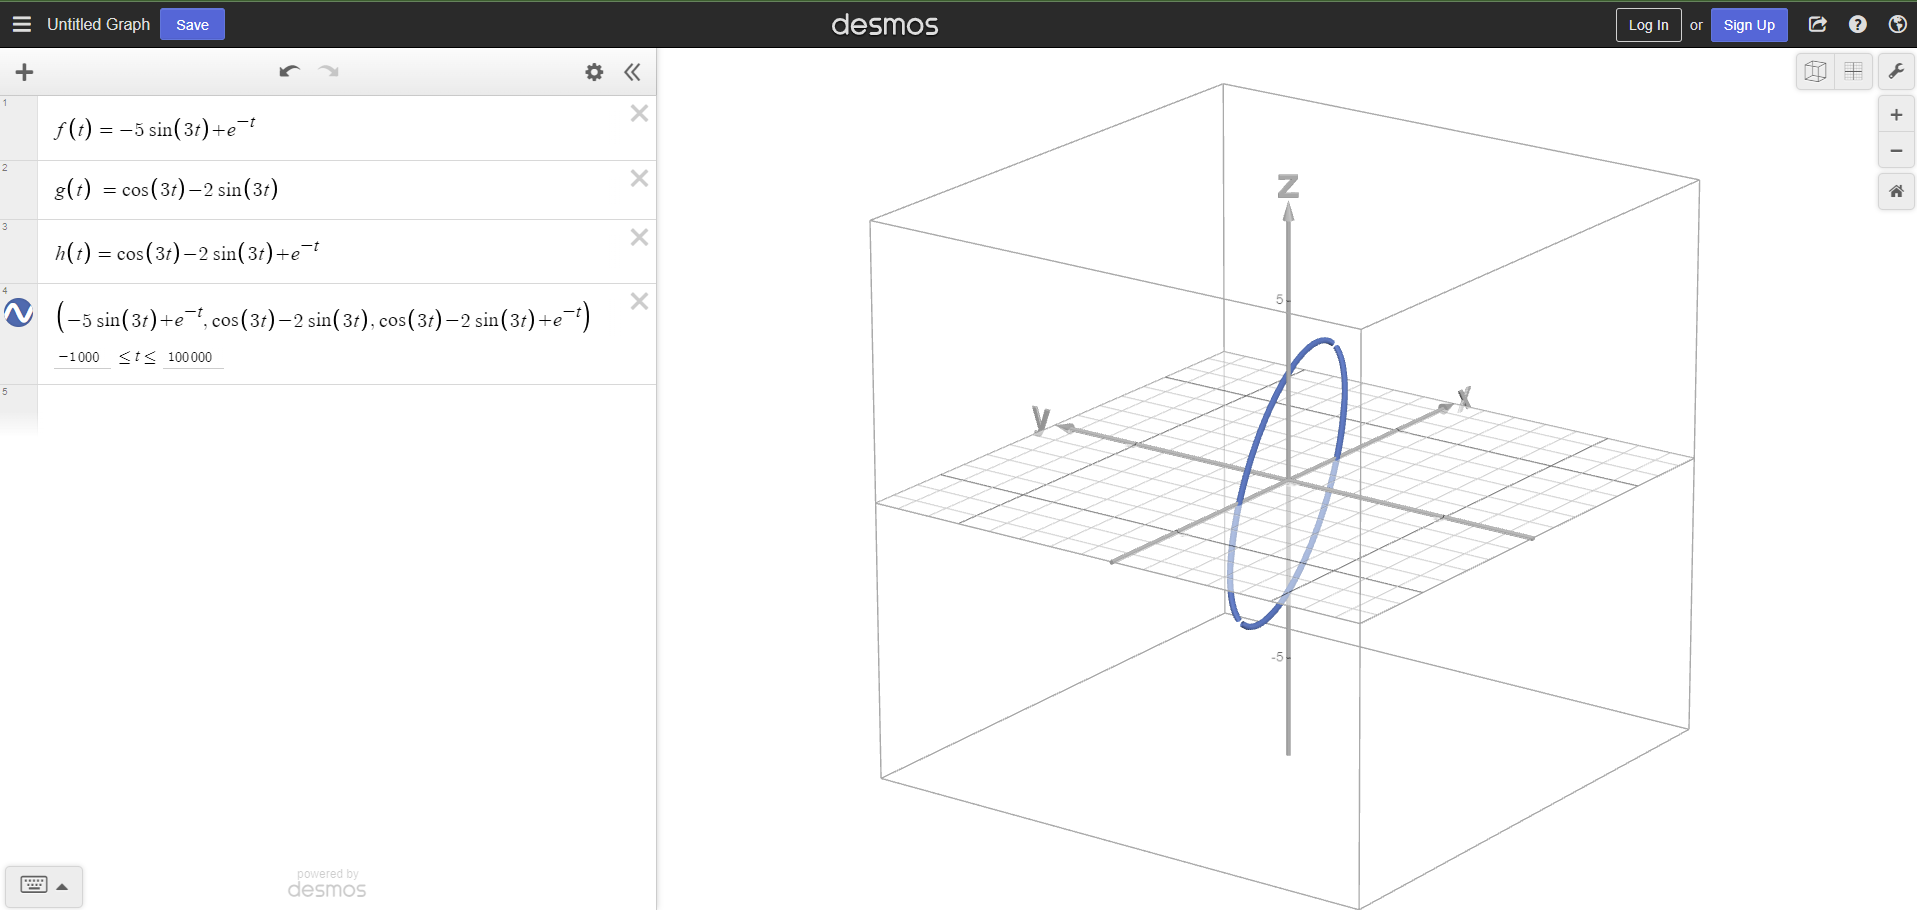
\includegraphics[width=0.7\textwidth]{Workshop_7.png}
\end{center}

\end{document}